\hypertarget{group__APU__STATUS__IS}{}\section{Status Value Tests}
\label{group__APU__STATUS__IS}\index{Status Value Tests@{Status Value Tests}}
Collaboration diagram for Status Value Tests\+:
\nopagebreak
\begin{figure}[H]
\begin{center}
\leavevmode
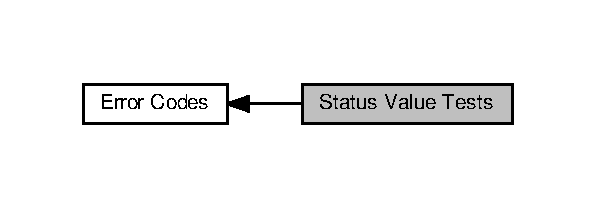
\includegraphics[width=286pt]{group__APU__STATUS__IS}
\end{center}
\end{figure}
\begin{DoxyWarning}{Warning}
For any particular error condition, more than one of these tests may match. This is because platform-\/specific error codes may not always match the semantics of the P\+O\+S\+IX codes these tests (and the corresponding A\+PR error codes) are named after. A notable example are the A\+P\+R\+\_\+\+S\+T\+A\+T\+U\+S\+\_\+\+I\+S\+\_\+\+E\+N\+O\+E\+NT and A\+P\+R\+\_\+\+S\+T\+A\+T\+U\+S\+\_\+\+I\+S\+\_\+\+E\+N\+O\+T\+D\+IR tests on Win32 platforms. The programmer should always be aware of this and adjust the order of the tests accordingly. 
\end{DoxyWarning}
